\chapter{ANÁLISES E RESULTADOS} % (fold)
\label{cha:analises_e_resultados}

\section{Introdução}
\label{sec:introducao}

 Para efetuar a análise dos resultados do experimento, inicialmente foram elaborados gráficos e tabelas com os valores obtidos da base de dados. Os seguintes dados foram considerados para a análise:
 
\begin{itemize}
	\item Grupos de usuários
	
	\subitem Utilizado para avaliar os laços de amizade entre os participantes cadastrados no experimento. São 12 grupos no total, sendo que cada um deles possui no máximo 5 pessoas.
	
	\item Recomendações enviadas por amigos
	
	\subitem Informações dos produtos que foram recomendados na etapa 3 do experimento, onde os participantes deveriam recomendar 5 produtos a cada amigo presente no seu grupo. Cada participante possui no máximo 20 recomendações, sendo que devido à desistência de participantes do seu grupo, alguns possuem apenas 15 recomendações.
	
	\item Recomendações enviadas por desconhecidos
	
	\subitem Informações dos produtos que foram recomendados na etapa 4 do experimento, onde os participantes deveriam recomendar 1 produto a alguns participantes de diferentes grupos, considerados desconhecidos. Cada participante possui no máximo 10 recomendações realizadas por desconhecidos, sendo que alguns, devido à desistência de participantes no experimento, possuem menos de 10 recomendações.
	
	\item Recomendações realizadas pelo sistema
	
	\subitem Todas as recomendações que o sistema realizou para os participantes. Contém a informação de qual participante recebeu a recomendação e qual foi o produto recomendado.
	
	\item Avaliação prevista do produto pelo sistema
	
	\subitem Ao recomendar um produto a um participante, o sistema calcula uma nota prevista para o mesmo. Essas informações foram armazenadas e consideradas durante a análise dos dados do experimento.
	
	\item Avaliações dos produtos
	
	\subitem Todas as avaliações de produtos no sistema. Contém os produtos avaliados na duas primeiras etapas do experimento, quando os participantes avaliaram 20 produtos em comum e 10 produtos de seu interesse, e as avaliações de produtos recomendados tanto pelos participantes como pelo sistema.  Lembrando que a escala de avaliação dos produtos é de 1 a 5, sendo 1 o participante não ter interesse e 5 o participante ter muito interesse naquele produto.
	
	\item Algoritmo utilizado para a recomendação
	
	\subitem Dentre as recomendações realizadas pelo sistema, foi retirada da base de dados a informação de qual algoritmo foi utilizado para gerar a recomendação.
	
\end{itemize}

 De posse dos dados, foram feitas as seguintes análises:
 
\begin{itemize}
	\item Análise Comparativa dos Algoritmos de Recomendação
	\item Análise de Rejeição das Recomendações
	\item Taxa de Serendipidade
	\item Análise do Algoritmo Baseado em Confiança
\end{itemize}

 Cada análise será discutida nas seções a seguir.
 
\section{Análise Comparativa dos Algoritmos de Recomendação}
\label{sec:analise_comparativa_dos_algoritmos_de_recomendacao}

Nesta seção, serão comparados os resultados dos três algoritmos de recomendação e as recomendações diretas feitas tanto por amigos quanto por desconhecidos.

\begin{figure}
    \centering
    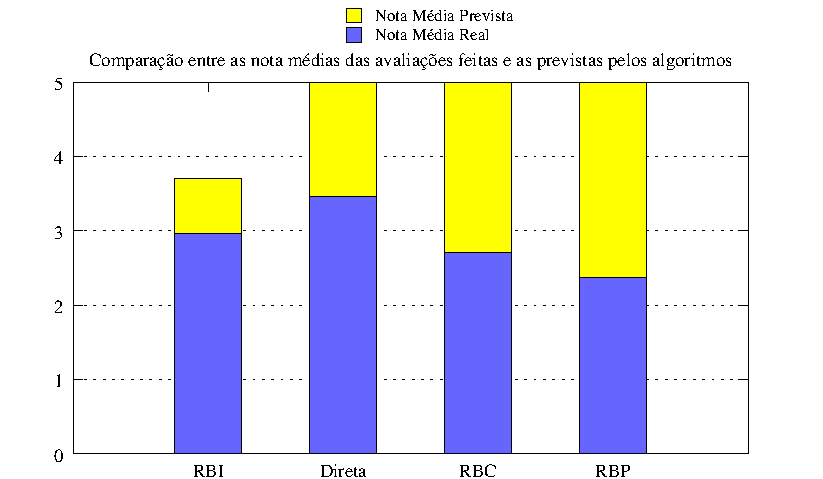
\includegraphics[width=\textwidth]{imagens/grafico_media_prevista}
    \caption{\it Nota média das avaliações realizadas comparadas com a nota média prevista pelos algoritmos}
    \label{fig:media_prevista}
\end{figure}
\begin{table}
\centering
\begin{tabular}{c c c}
    \hline
    \hline
    \textbf{Tipo de recomendação} & \textbf{Nota Média}& \textbf{Nota Média Prevista} \\
    \hline 
RBI & 2.964 & 3.70 \\

\hline 
Direta & 3.46 & 5.00 \\
\hline 
RBC & 2.70 & 5.00 \\
\hline 
RBP & 2.37 & 5.00 \\
\hline        
\end{tabular}
\caption{\it Nota média das avaliações realizadas comparadas com a nota média prevista pelos algoritmos}
\label{table:media_prevista}
\end{table}

A Figura~\ref{fig:media_prevista} compara a média da nota prevista com a nota média real dada pelos participantes do sistema. A Tabela~\ref{table:media_prevista} contém os dados utilizados para a construção do gráfico. Nota-se que o algoritmos RBC e RBP deram nota 5 para todos os produtos recomendados, resultando em uma grande diferença em relação à avaliação real. O RBI consegue fazer uma previsão bem próxima da real, mostrando que o seu modelo das avaliações é bastante preciso. Para as recomendações diretas, foi considerado que uma pessoa ao recomendar espera que a recomendação seja avaliada com nota máxima, resultando em uma nota prevista 5.

 As notas médias dadas pelos participantes estão discriminadas por algoritmos de recomendação e pelas recomendações diretas, como mostra a Figura~\ref{fig:notas_medias}. Os dados utilizados para a elaboração do gráficos estão na Tabela~\ref{table:notas_medias}. As recomendações que resultaram em uma média de notas maior foram as diretas, seguidas das realizadas com o algoritmo RBI, RBC e RBP.
 
\begin{figure}
    \centering
    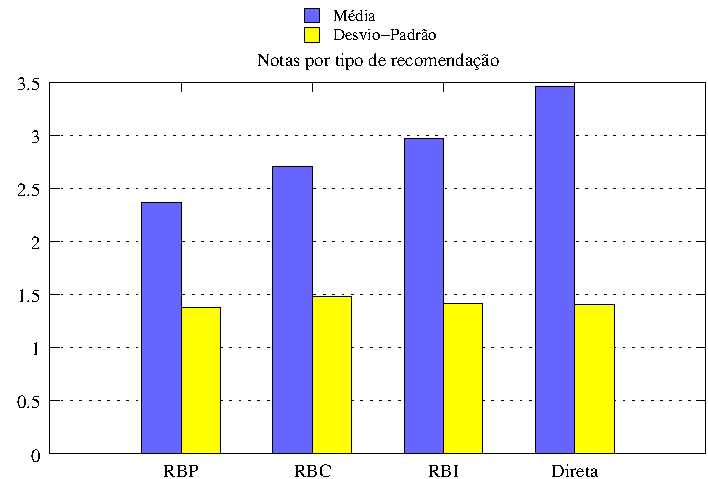
\includegraphics[width=\textwidth]{imagens/grafico_notas_medias}
    \caption{\it Notas por tipo de recomendação}
    \label{fig:notas_medias}
\end{figure}

\begin{table}
\centering
\begin{tabular}{c c c}
    \hline \hline
    \textbf{Tipo de recomendação} & \textbf{Média}& \textbf{Desvio-Padrão} \\
\hline 
Direta & 3.46 & 1.41 \\
\hline 
RBC & 2.70 & 1.48 \\
\hline 
RBI & 2.96 & 1.41 \\
\hline 
RBP & 2.37 & 1.38 \\
\hline        
\end{tabular}
\caption{\it Notas por tipo de recomendação}
\label{table:notas_medias}
\end{table}

 As notas médias dadas por recomendações diretas foram separadas entre as realizadas por amigos e as feitas por desconhecidos, como ilustra a Figura~\ref{fig:notas_medias_diretas}. Os dados utilizados para a construção do gráfico está na Tabela~\ref{table:notas_medias_diretas}. Verifica-se que a média de notas dadas por recomendações realizadas por amigos foi ligeiramente maior que as notas dadas a produtos indicados por desconhecidos.

\begin{figure}
    \centering
    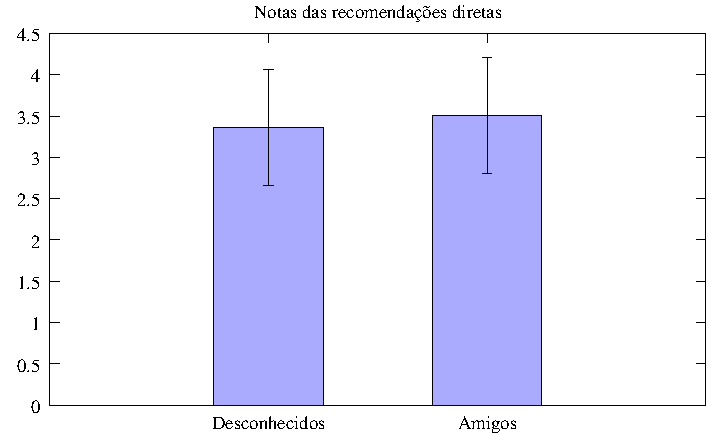
\includegraphics[width=\textwidth]{imagens/grafico_notas_medias_diretas}
    \caption{\it Notas das recomendações diretas}
    \label{fig:notas_medias_diretas}
\end{figure}

\begin{table}
\centering
\begin{tabular}{c c c}
    \hline \hline
    \textbf{Tipo de recomendação} & \textbf{Média}& \textbf{Desvio-Padrão} \\
\hline 
Amigos & 3.51 & 1.41 \\
\hline 
Desconhecidos & 3.36 & 1.40 \\
\hline        
\end{tabular}
\caption{\it Notas das recomendações diretas}
\label{table:notas_medias_diretas}
\end{table}

% section analise_comparativa_dos_algoritmos_de_recomendacao (end)

\section{Análise de Rejeição das Recomendações}
\label{sec:analise_de_rejeicao_das_recomendacoes}

 Nesta seção, serão analisadas a taxa de rejeição das recomendações realizadas pelos algoritmos RBI, RBP e RBC, além das recomendações diretas. Para isso, foram definidas classes de avaliações. As avaliações com notas 1 e 2 são da classe de \textit{Rejeição}, as com nota 3 são da classe \textit{Indiferente} e as com notas 4 e 5 são da classe \textit{Aceitação}. A classe Rejeição denota as recomendação que não foram aceitas e a classe Aceitação denota as recomendações que foram aceitas. Na classe Indiferente, estão as recomendações que tiveram avaliações neutras (nota 3).

 Podemos verificar pela Figura~\ref{fig:notas} que as recomendações diretas representaram uma maior porcentagem de notas na classe de Aceitação, seguida das recomendações feitas pelo algoritmo RBI, RBC e, por fim, RBP. Os dados utilizados para a elaboração do gráfico constam na Tabela~\ref{table:notas}.
%TODO concluir análise
 
\begin{figure}
    \centering
    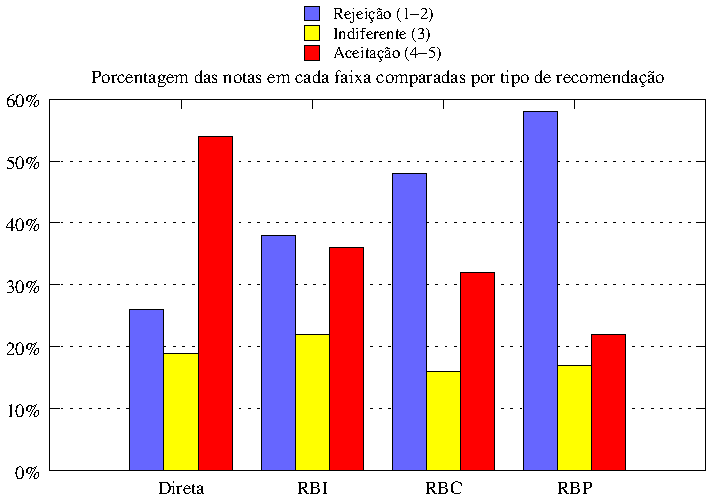
\includegraphics[width=\textwidth]{imagens/grafico_notas}
    \caption{\it Porcentagem das notas em cada faixa comparadas por tipo de recomendação}
    \label{fig:notas}
\end{figure}

\begin{table}
\centering
\begin{tabular}{c c c c} 
    \hline \hline
    \textbf{Tipo de recomendação} & \textbf{Rejeição}& \textbf{Indiferente}& \textbf{Aceitação} \\
\hline 
Direta & 26\% & 19\% & 54\% \\
\hline 
RBC & 48\% & 16\% & 32\% \\
\hline 
RBI & 38\% & 22\% & 36\% \\
\hline 
RBP & 58\% & 17\% & 22\% \\
\hline        
\end{tabular}
\caption{\it Porcentagem das notas em cada faixa comparadas por tipo de recomendação}
\label{table:notas}
\end{table}

% section analise_de_rejeicao_das_recomendacoes (end)

\section{Taxa de Serendipidade}
\label{sec:taxa_de_serendipidade}

Serendipidade significa o usuário ter aceito a recomendação, ou seja, ter dado uma nota 4 ou 5 ao produto e não o conhecer. A taxa de serendipidade foi calculada com base no número de recomendações de produtos desconhecidos aceitas sobre o total de produtos recomendados em cada tipo de algoritmo, considerando também as recomendações diretas. A Figura~\ref{fig:serendipidade} mostra a taxa de serendipidade para os tipos de recomendação, sendo que os dados utilizados para elaborar o gráfico estão na Tabela~\ref{table:serendipidade}.

Verificamos que as recomendações diretas resultaram em um alto grau de serendipidade, se comparado com os graus dos tipos de recomendações que as seguiram: RBI, RBC e RBP.

\begin{figure}
    \centering
    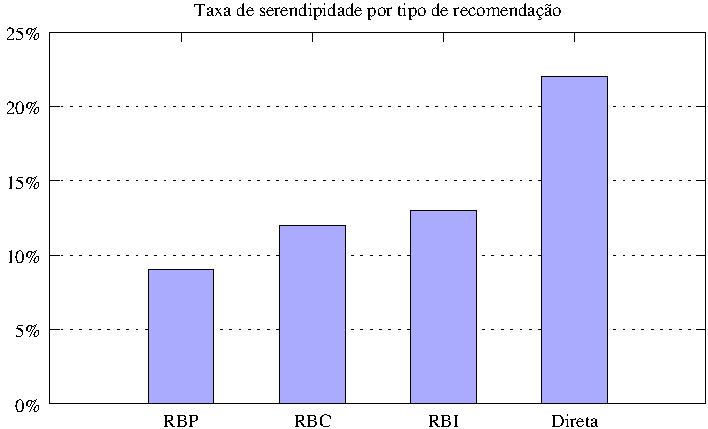
\includegraphics[width=\textwidth]{imagens/grafico_serendipidade}
    \caption{\it Taxa de serendipidade por tipo de recomendação}
    \label{fig:serendipidade}
\end{figure}

\begin{table}
\centering
\begin{tabular}{c c}
    \hline \hline
    \textbf{Tipo de recomendação} & \textbf{Taxa de Serendipidade} \\
\hline 
Direta & 22\% \\
\hline 
RBC & 12\% \\
\hline 
RBI & 13\% \\
\hline 
RBP & 9\% \\
\hline        
\end{tabular}
\caption{\it Taxa de serendipidade por tipo de recomendação}
\label{table:serendipidade}
\end{table}

A Figura~\ref{fig:serendipidade_diretas} compara a taxa de serendipidade entre as recomendações diretas realizadas por amigos e por desconhecidos. A Tabela~\ref{table:serendipidade_diretas} contém os dados utilizados para elaborar o gráfico. Podemos ver que as recomendações realizadas pelos amigos resultaram em uma taxa de serendipidade ligeiramente maior que as recomendações realizadas por desconhecidos.
%TODO concluir análise

\begin{figure}
    \centering
    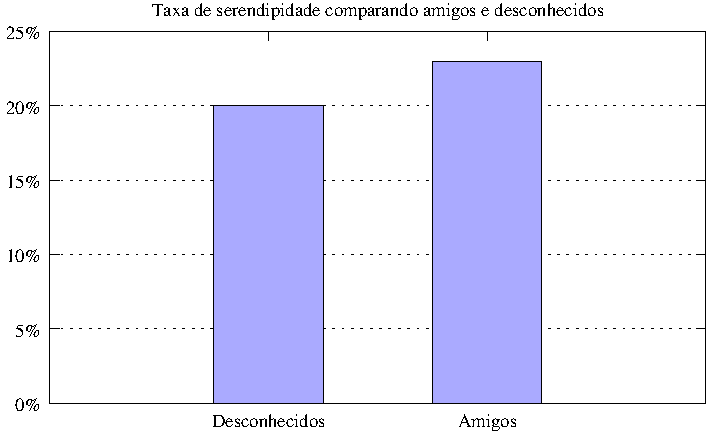
\includegraphics[width=\textwidth]{imagens/grafico_serendipidade_diretas}
    \caption{\it Taxa de serendipidade comparando amigos e desconhecidos}
    \label{fig:serendipidade_diretas}
\end{figure}

\begin{table}
\centering
\begin{tabular}{c c}
    \hline \hline
    \textbf{Tipo de recomendação} & \textbf{Taxa de Serendipidade} \\
\hline 
Amigos & 23\% \\
\hline 
Desconhecidos & 20\% \\
\hline        
\end{tabular}
\caption{\it Taxa de serendipidade comparando amigos e desconhecidos}
\label{table:serendipidade_diretas}
\end{table}

% section taxa_de_serendipidade (end)

\section{Análise do Algoritmo Baseado em Confiança}
\label{sec:analise_do_algoritmo_baseado_em_confianca}

 Com os dados apresentados na seções anteriores, podemos verificar que o algoritmo de recomendação baseado em confiança (RBC) produziu. em alguns casos, resultados relativamente melhores do que o algoritmo RBP.
 
 Na análise de desvio da nota prevista, o RBC não foi tão eficiente quanto as recomendações diretas e o algoritmo RBI, porém mostrou resultados melhores que o RBP. 
 
 Verificando a média de notas dadas, o RBC teve resultado intermediário com relação aos outros dois algoritmos, sendo que as recomendações diretas apresentaram a melhor eficiência. Isso ocorreu principalmente pelo fato dos desconhecidos terem recomendado quase tão bem como os amigos, como mostra a Figura~\ref{fig:notas_medias_diretas}.
 
 Quanto à taxa de serendipidade, o RBC manteve-se na média dos outros algoritmos, sendo que as recomendações diretas foram disparadamente mais eficientes.
 
 De acordo com os dados, o RBC conseguiu recomendar melhor que o RBP. O RBC utiliza menos informações que o RBP, limitando-se aos usuários que realizaram recomendações ao usuário alvo, para recomendar e mesmo assim mostrou-se melhor nos resultados do experimento.

% section analise_do_algoritmo_baseado_em_confianca (end)

\section{Testes de Hipótese}

Um dos objetivos do experimento foi testar certas hipóteses que, ao serem confirmadas, fornecem uma base mais sólida para a construção de sistemas de recomendação efetivos.

A seguir cada hipótese será analisada. As hipóteses nulas (H0) são todas iguais, elas consideram que as duas diferentes distribuições pouco diferem, tendo por exemplo a mesma média, mediana ou algum critério equivalente que depende exatamente do teste de hipótese utilizado. Para mais informações, consultar a seção apêndice~\ref{anexo_hipoteses}, onde estão listados os testes utilizados e os resultados numéricos dos mesmos.

\subsubsection{TH1: Os Amigos Recomendam Melhor do que os Desconhecidos}
A hipótese nula foi rejeitada com um nível de significância de 10\%, confirmando esta hipótese quando também se considera que a média das recomendações dos amigos é maior do que as dos desconhecidos, conforme pode ser visto na figura~\ref{fig:notas_medias_diretas}.


\subsubsection{TH2: A Recomendação Baseada em Confiança é Melhor do que a Baseada em Similaridade de Perfil dos Usuários}
A hipótese nula foi rejeitada com um nível de significância de 0.5\%, confirmando a hipótese de que o algoritmo apresentado nesta monografia (RBC) tem um desempenho superior ao algoritmo de similaridade de perfil (RBP), que é um dos mais utilizados na filtragem social. As figuras \ref{fig:notas} e \ref{fig:notas_medias} mostram a melhor aceitação da RBC em relação a RBP.

\subsubsection{TH3: As Recomendações Diretas são Melhores do que as Baseadas em Confiança}
A hipótese nula foi rejeitada com um nível de significância de 0.5\%, confirmando que as recomendações feitas diretamente pelas pessoas possuem uma aceitação muito maior do que o algoritmo apresentado neste trabalho, como pode ser visto nas figuras~\ref{fig:notas} e \ref{fig:notas_medias}.

\subsubsection{TH4: As Recomendações Baseadas em Similaridade de Itens são Melhores do que as Baseadas em Confiança}
A hipótese nula foi rejeitada com um nível de significância de 0.5\%, confirmando, como pode ser visto nas figuras \ref{fig:notas} e \ref{fig:notas_medias}, que a RBI é melhor aceita do que a RBC.

\begin{figure}
    \centering
    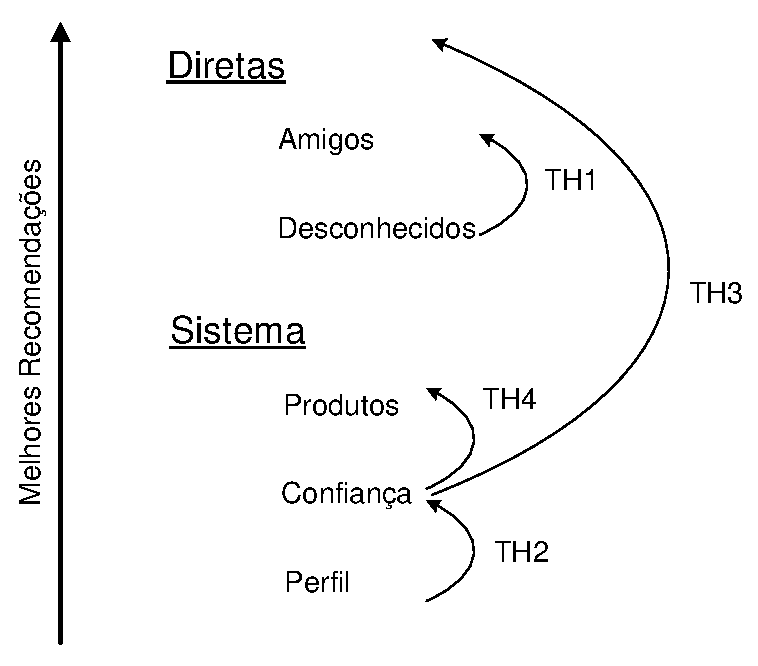
\includegraphics[width=\textwidth]{imagens/testes}
    \caption{\it Resultado dos testes de hipótese}
    \label{fig:testes}
\end{figure}

 Tais testes de hipótese são mostrados na Figura~\ref{fig:testes}.

\section{Análise de Desempenho}
\label{sec:analise_de_desempenho}
% TODO falar sobre os problemas enfrentados com as consultas SQL e com as estrelinhas para a avaliação do produto (javascript).
Durante a realização do experimento foram evidenciados problemas de desempenho que prejudicavam a experiência dos participantes. Sendo assim, surgiu a necessidade de realizar uma análise de desempenho para encontrar os gargalos do sistema e modificá-los de modo a reduzir o tempo de resposta a um nível aceitável pelo usuário.

Algumas requisições ao servidor de aplicação foram identificadas como gargalo de desempenho do sistema, como pode se observar na Tabela~\ref{table:before_stats}. Ao analisar estas requisições, foi possível verificar que os principais fatores responsáveis pela degradação do desempenho estavam relacionados ao tempo e quantidade das requisições ao banco de dados. As consultas SQL na tabela de produtos, com cerca de cento e vinte mil registros, foram as principais responsáveis pelo excesso no tempo de resposta. Esses problemas de desempenho foram corrigidos através da redução do número de requisições ao banco de dados e pela paginação dos resultados. Os tempos de resposta das requisições observados após a otimização estão apresentados na Tabela~\ref{table:after_stats}.

\begin{table}\centering
\begin{tabular}{c c c c c}
\hline \hline
\textbf{Requisição Web}
& \textbf{Média}
& \textbf{Desvio Padrão}
& \textbf{Min.} 
& \textbf{Max.} \\ \hline
ProductsController\#index.html [GET]    & 16.90s & 29.02s &  0.00s &  5m06s \\
\hline
ProductsController\#rate.html [POST]    &  2.09s &  1.24s &  0.80s & 32.16s \\
\hline
ProductsController\#unknown.html [POST] &  1.26s &  0.54s &  0.85s &  2.42s \\
\hline
ProductsController\#show.html [GET]     &  1.18s &  1.21s &  0.00s &  8.52s \\
\hline
\end{tabular}
\caption{\it Tempo de resposta das requisições ao banco de dados antes da otimização \label{table:before_stats}}
\end{table}

\begin{table}\centering
\begin{tabular}{c c c c c}
\hline \hline
\textbf{Requisição Web}
& \textbf{Média}
& \textbf{Desvio Padrão}
& \textbf{Min.} 
& \textbf{Max.} \\ \hline
ProductsController\#index.html [GET]    & 1.28s &  3.51s &  0.00s & 57.42s \\
\hline
ProductsController\#rate.html [POST]    & 0.13s &  0.77s &  0.00s & 21.05s \\
\hline
ProductsController\#unknown.html [POST] & 0.02s &  0.10s &  0.00s &  2.66s \\
\hline
ProductsController\#show.html [GET]     & 0.02s &  0.12s &  0.00s &  1.99s \\
\hline
\end{tabular}
\caption{\it Tempo de resposta das requisições ao banco de dados após a otimização \label{table:after_stats}}
\end{table}

Para completar a análise do desempenho do sistema, a Tabela~\ref{table:process_blockers} apresenta as requisições bloqueantes, isto é, aquelas com duração total maior do que um segundo. Os dados apresentados na Tabela~\ref{table:process_blockers} são referentes apenas as requisições feitas após a otimização até o término do experimento.

\begin{table}\centering
\begin{tabular}{c c c}
\hline \hline
\textbf{Requisição Web}
& \textbf{Ocorrências}
& \textbf{Porcentagem} \\ \hline
UserRecommendationsController\#new.html [GET]     & 1596 & 65.2\% \\ 
\hline
ProductsController\#index.html [GET]              &  315 & 12.9\% \\ 
\hline
AdminController\#index.html [GET]                 &  167 &  6.8\% \\
\hline
ProductsController\#rate.html [POST]              &  165 &  6.7\% \\
\hline
HomeController\#index.html [GET]                  &  128 &  5.2\% \\ 
\hline
UserRecommendationsController\#create.html [POST] &   38 &  1.6\% \\
\hline
RecommendationGuidesController\#index.html [GET]  &   11 &  0.4\% \\  
\hline
InvitationsController\#create.html [POST]         &    8 &  0.3\% \\  
\hline
ProductsController\#unknown.html [POST]           &    8 &  0.3\% \\  
\hline
RatingsController\#index.html [GET]               &    7 &  0.3\% \\  
\hline
SessionsController\#create.html [POST]            &    4 &  0.2\% \\  
\hline
UsersController\#new.html [GET]                   &    1 &  0.0\% \\  
\hline
ProductsController\#show.html [GET]               &    1 &  0.0\% \\
\hline
\end{tabular}
\caption{\it Requisições bloqueantes \label{table:process_blockers}}
\end{table}


% section analise_de_desempenho (end)
